\section*{NAIL062 P\&P Logic: Worksheet 1 -- Intro to propositional logic}
% after Lecture 1

\subsection*{Teaching goals:} After completing, the student

    \begin{itemize}\setlength{\itemsep}{0pt}
        \item understands the notions of propositional logic syntax (language, atomic proposition, proposition, tree of a proposition, subproposition, theory), formally define them and give examples
        \item understands the notions of model, consequence of a theory, formally define them and give examples
        \item can formalize a given system (word/computational problem, etc.) in propositional logic
        \item can find models of a given theory
        \item can decide whether a given proposition is a consequence of a given theory
        \item has experience applying (with instructor assistance) the tableau method and resolution method to prove properties of a given system (e.g., to solve a word problem)
    \end{itemize}


\section*{In-class problems}


\begin{problem}\label{problem:dragons}
    
    We got lost in a labyrinth and in front of us are three doors: red, blue, and green. We know that behind exactly one of the doors there is the way out, behind the others there is a dragon. On the doors there are inscriptions:
    \begin{itemize}
        \item Red door: {\it ``The way out is behind this door.''}
        \item Blue door: {\it ``The way out is not behind this door.''}
        \item Green door: {\it ``The way out is not behind the blue door.''}
    \end{itemize}
    We know that at least one of the inscriptions is true and at least one is false. Which way leads out?
    \begin{enumerate}[(a)]
        \item Choose a suitable language (a set of propositional variables) $\mathbb P$.
        \item Formalize all knowledge as a theory $T$ in the language $\mathbb P$. (Note: The axioms are not the inscriptions on the doors; those need not be true.)
        \item Find all models of the theory $T$.
        \item Formalize the statements ``The way out is behind the red/blue/green door'' as formulas $\varphi_1,\varphi_2,\varphi_3$ over $\mathbb P$. Is any of these formulas a consequence of $T$?
        \item Try using the tableau method: Construct a tableau from the theory $T$ with the item $F\varphi_i$ at the root. Will all branches be contradictory? (Try to come up with the correct steps for the construction of the tableau, take inspiration from the example in the lecture.)
        \item Try using the resolution method: Convert the axioms of the theory $T$, as well as the formula $\neg\varphi_i$, into conjunctive normal form (CNF). Try to construct a resolution refutation and draw it in the form of a resolution tree. (Note: Don’t forget to negate the formula $\varphi_i$ you are proving.)
    \end{enumerate}  

    \begin{solution}
        \begin{enumerate}[(a)]
            \item A natural choice is the language $\mathbb P=\{p_1, p_2, p_3\}$, where $p_i$ means `the way out is behind the $i$-th door', with the doors ordered red, blue, green as in the assignment. (We could also have used `there is a dragon behind the $i$-th door' or `the inscription on the $i$-th door is true'. The important thing is that the chosen language is as small as possible. If we have $p_i$, we can for example express `there is a dragon behind the $i$-th door' as `$\neg p_i$', so we don’t need another propositional variable. Furthermore, we want the properties from the assignment to be as easy to formalize as possible.)
            \item From the assignment we understand that `there is a dragon' means the same as `there is no way out'. The fact that the way out is behind exactly one of the doors can be expressed by saying that it is behind at least one door, and for each pair of doors it is not behind both:
            $$
            \alpha_1=(p_1\lor p_2\lor p_3) \land (\neg p_1\lor\neg p_2) \land  (\neg p_1\lor\neg p_3) \land (\neg p_2\lor\neg p_3)
            $$
            Now for the inscriptions on the doors, first let’s formalize their meaning:
            \begin{itemize}
                \item Red door: ``$p_1$''
                \item Blue door: ``$\neg p_2$''
                \item Green door: ``$\neg p_2$''
            \end{itemize}
            At least one of these inscriptions is true: $p_1\lor \neg p_2\lor\neg p_2$, which simplifies to
            $$
            \alpha_2=p_1\lor \neg p_2
            $$
            Similarly, the fact that at least one of the inscriptions is false can be formalized as $\neg p_1\lor \neg \neg p_2\lor\neg \neg p_2$, which after simplification (think about why this is equivalent) gives:
            $$
            \alpha_3=\neg p_1\lor p_2
            $$
            The resulting theory is thus:
            \begin{align*}
                T=\{&\alpha_1,\alpha_2,\alpha_3\}\\=\{&(p_1\lor p_2\lor p_3) \land (\neg p_1\lor\neg p_2) \land  (\neg p_1\lor\neg p_3) \land (\neg p_2\lor\neg p_3), p_1\lor \neg p_2, \neg p_1\lor p_2\}
            \end{align*}
            \item Later we will learn to find models using the tableau method, but for now an `inefficient' procedure: First we find the models of one axiom. Since the first axiom is rather complicated, it may be better to start with axiom $\alpha_2$. (In principle, we could try all 8 models of the language $\mathbb P$, and for each of them compute the truth value of $\alpha_2$.) We obtain:
            $$
            \M_\mathbb P(\alpha_2)=\{(0,0,0),(0,0,1),(1,0,0),(1,0,1),(1,1,0),(1,1,1)\}
            $$
            Now we check in which of these models axiom $\alpha_3$ holds:
            $$
            \M_\mathbb P(\alpha_2,\alpha_3)=\{(0,0,0),(0,0,1),(1,1,0),(1,1,1)\}
            $$
            Finally, we check the validity of $\alpha_1$ in each of these 4 models:
            $$
            \M_\mathbb P(T)=\M_\mathbb P(\alpha_1,\alpha_2,\alpha_3)=\{(0,0,1)\}
            $$
            \item With our choice of language $\mathbb P$ the formalization is simple: $\varphi_1=p_1$, $\varphi_2=p_2$, $\varphi_3=p_3$. Being a consequence of theory $T$ means holding in every model of $T$ (note: in every model, not just `in some model’---this is a common mistake). In our case, $T$ has only one model, and we immediately see that $\varphi_3$ holds in it while $\varphi_1$ and $\varphi_2$ do not. Thus, the only consequence of $T$ among these is $\varphi_3$.
            \item When using the tableau method, we proceed as in the introductory chapter of the lecture notes (Section 1.1.5). To prove that $\varphi_3$ holds in $T$, we construct a tableau from the theory $T$, where we put the assumption $\mathrm{F}p_3$ at the root, since we are proving by contradiction ($\mathrm{F}$ means `False’, $\mathrm{T}$ means `True’). 
            
            Recall that we expand a tableau by attaching assumptions about the validity of the axioms $\mathrm{T}\alpha_i$ ($i\in\{1,2,3\}$) and by reducing items (attaching the corresponding atomic tableaux). The order in which we do this can significantly affect the size of the resulting tableau proof. It is good first to reduce items whose atomic tableaux do not branch, or that do branch but one of the branches immediately becomes contradictory. We attach the axioms only when needed. It is often helpful to think through how we would proceed in the proof ourselves, and then build the tableau accordingly.

            Note also that we do not define atomic tableaux for conjunctions or disjunctions of three or more formulas. (We want the algorithm steps to be as simple as possible.) For example, in $\mathrm{T}p_1\lor p_2\lor p_3$, we first imagine the omitted parentheses, $\mathrm{T}p_1\lor (p_2\lor p_3)$, and then reduce in two steps by attaching $\mathrm{T}p_1$ and $\mathrm{T}p_2\lor p_3$:
            
            \begin{center}
                \begin{forest}
                    [$\mathrm{T}p_1\lor (p_2\lor p_3)$
                        [$\mathrm{T}p_1$]
                        [$\mathrm{T}p_2\lor p_3$
                            [$\mathrm{T}p_2$]
                            [$\mathrm{T}p_3$]
                        ]
                    ]            
                \end{forest}
            \end{center}

            (We also note that from the perspective of the tableau method it would be a bit better to have, instead of axiom $\alpha_1$, four separate formulas whose conjunction it is. This would shorten the tableau construction. But the algorithm can handle axioms of any complexity.)

            Here is one possible tableau proof ($\oplus$ marks a contradictory branch, $\checkmark$ a completed consistent one). At first glance it may look complicated, but in fact we are just running a simple algorithm. Work out where each item came from and where we see atomic tableaux:
            
            \begin{center}
                \begin{forest}
                    [$\mathrm{F}p_3$
                        [$\mathrm{T}(p_1\lor p_2\lor p_3) \land ((\neg p_1\lor\neg p_2) \land  (\neg p_1\lor\neg p_3) \land (\neg p_2\lor\neg p_3))$
                            [$\mathrm{T}p_1\lor (p_2\lor p_3)$
                                [$\mathrm{T}(\neg p_1\lor\neg p_2) \land  ((\neg p_1\lor\neg p_3) \land (\neg p_2\lor\neg p_3))$
                                    [$\mathrm{T}\neg p_1\lor\neg p_2$
                                        [$\mathrm{T}(\neg p_1\lor\neg p_3) \land (\neg p_2\lor\neg p_3)$
                                            [$\mathrm{T}\neg p_1\lor\neg p_3$
                                                [$\mathrm{T}\neg p_2\lor\neg p_3$
                                                    [$\mathrm{T}p_1\lor \neg p_2$
                                                        [$\mathrm{T}p_1$
                                                            [$\mathrm{T}\neg p_1\lor p_2$
                                                                [$\mathrm{T}\neg p_1$
                                                                    [$\mathrm{F}p_1$, tikz={\node[fit to=tree,label=below:$\otimes$] {};}]
                                                                ]
                                                                [$\mathrm{T}p_2$
                                                                    [$\mathrm{T}\neg p_1$
                                                                        [$\mathrm{F}p_1$, tikz={\node[fit to=tree,label=below:$\otimes$] {};}]
                                                                    ]
                                                                    [$\mathrm{T}\neg p_2$
                                                                        [$\mathrm{F}p_2$, tikz={\node[fit to=tree,label=below:$\otimes$] {};}]
                                                                    ]
                                                                ]
                                                            ]
                                                        ]
                                                        [$\mathrm{T}\neg p_2$
                                                            [$\mathrm{F}p_2$
                                                                [$\mathrm{T}\neg p_1\lor p_2$
                                                                    [$\mathrm{T}\neg p_1$
                                                                        [$\mathrm{F}p_1$
                                                                            [$\mathrm{T}p_1$, tikz={\node[fit to=tree,label=below:$\otimes$] {};}]
                                                                            [$\mathrm{T}p_2\lor p_3$
                                                                                [$\mathrm{T}p_2$, tikz={\node[fit to=tree,label=below:$\otimes$]{};}]
                                                                                [$\mathrm{T}p_3$, tikz={\node[fit to=tree,label=below:$\otimes$]{};}]
                                                                            ]
                                                                        ]
                                                                    ]
                                                                    [$\mathrm{T}p_2$, tikz={\node[fit to=tree,label=below:$\otimes$] {};}]
                                                                ]          
                                                            ]
                                                        ]    
                                                    ]    
                                                ]
                                            ]    
                                        ]
                                    ]
                                ]
                            ]
                        ]
                    ]  
                \end{forest}
            \end{center}
            
            What if we tried to prove $p_1$ or $p_2$ from theory $T$? Let’s show it for $p_1$ (try $p_2$ yourself). We put $\mathrm{F}p_1$ at the root. We proceed analogously, but at least one branch will remain consistent even after completion (adding all axioms and reducing all items). From the consistent branches we can then read off a counterexample (a model of $T$ in which $p_1$ does not hold).

            Below is a completed tableau. Verify that all axioms are used and all items reduced. We get two completed consistent branches. Looking at the assumptions about propositional variables on them: in both we have $\mathrm{F}p_1$, $\mathrm{F}p_2$, $\mathrm{T}p_3$. This corresponds to the model $(0,0,1)$, which is indeed a counterexample: a model of $T$ in which $p_1$ does not hold.

            \begin{center}
                \begin{forest}
                    [$\mathrm{F}p_1$
                        [$\mathrm{T}p_1\lor\neg p_2$
                            [$\mathrm{T}p_1$, tikz={\node[fit to=tree,label=below:$\otimes$] {};}]
                            [$\mathrm{T}\neg p_2$
                                [$\mathrm{F}p_2$
                                    [$\mathrm{T}(p_1\lor p_2\lor p_3) \land ((\neg p_1\lor\neg p_2) \land  (\neg p_1\lor\neg p_3) \land (\neg p_2\lor\neg p_3))$
                                        [$\mathrm{T}p_1\lor (p_2\lor p_3)$
                                            [$\mathrm{T}(\neg p_1\lor\neg p_2) \land  ((\neg p_1\lor\neg p_3) \land (\neg p_2\lor\neg p_3))$
                                                [$\mathrm{T}p_1$, tikz={\node[fit to=tree,label=below:$\otimes$] {};}]
                                                [$\mathrm{T}p_2\lor p_3$
                                                    [$\mathrm{T}p_2$, tikz={\node[fit to=tree,label=below:$\otimes$]{};}]
                                                    [$\mathrm{T}p_3$
                                                        [$\mathrm{T}\neg p_1\lor\neg p_2$
                                                            [$\mathrm{T}(\neg p_1\lor\neg p_3) \land (\neg p_2\lor\neg p_3)$
                                                                [$\mathrm{T}\neg p_1\lor\neg p_3$
                                                                    [$\mathrm{T}\neg p_2\lor\neg p_3$
                                                                        [$\mathrm{T}\neg p_1$
                                                                            [$\mathrm{F}p_1$
                                                                                [$\mathrm{T}\neg p_2$
                                                                                    [$\mathrm{F}p_2$
                                                                                        [$\mathrm{T}\neg p_1\lor p_2$
                                                                                            [$\mathrm{T}\neg p_1$
                                                                                                [$\mathrm{F}p_1$
                                                                                                    [$\mathrm{T}\neg p_1$
                                                                                                        [$\mathrm{F}p_1$, tikz={\node[fit to=tree,label=below:$\checkmark$] {};}]
                                                                                                    ]
                                                                                                    [$\mathrm{T}\neg p_2$
                                                                                                        [$\mathrm{F}p_2$, tikz={\node[fit to=tree,label=below:$\checkmark$] {};}]
                                                                                                    ]
                                                                                                ]
                                                                                            ]
                                                                                            [$\mathrm{T}p_2$, tikz={\node[fit to=tree,label=below:$\otimes$] {};}]
                                                                                        ]
                                                                                    ]
                                                                                ]
                                                                                [$\mathrm{T}\neg p_3$
                                                                                    [$\mathrm{F}p_3$, tikz={\node[fit to=tree,label=below:$\otimes$] {};}]
                                                                                ]
                                                                            ]
                                                                        ]
                                                                        [$\mathrm{T}\neg p_3$
                                                                            [$\mathrm{F}p_3$, tikz={\node[fit to=tree,label=below:$\otimes$] {};}]
                                                                        ]
                                                                    ]
                                                                ]    
                                                            ]
                                                        ]                                                
                                                    ]
                                                ]
                                            ]
                                        ]
                                    ]
                                ]
                            ]
                        ]
                    ]
                \end{forest}
            \end{center}

            \item When using the resolution method, we proceed as in the introductory chapter of the lecture notes, in Section 1.1.6. To prove that $p_3$ holds in $T$, we add to the theory $T$ the formula $\neg p_3$ as an axiom. We thus have $T'=\{\alpha_1,\alpha_2,\alpha_3,\neg p_3\}$. Using equivalence transformations we convert into CNF (express as a conjunction of clauses, i.e., disjunctions of literals). In our case all axioms are already in CNF ($\alpha_1$ is a conjunction of three clauses, the others are clauses themselves). The resulting CNF formula, written in set notation (for clarity it is good to write the literals in a fixed order), is:
            $$
            S=\{\{p_1,p_2,p_3\},\{\neg p_1,\neg p_2\},\{\neg p_1,\neg p_3\},\{\neg p_2,\neg p_3\},\{p_1,\neg p_2\},\{\neg p_1,p_2\},\{\neg p_3\}\}
            $$
            Now we construct a resolution refutation. How do we choose the resolution steps? A good heuristic is that a shorter clause contains more information. So we try to start from the shortest clauses, here $\{\neg p_3\}$, and see where we can use newly derived (`learned’) clauses. A clause often needs to be used repeatedly. Here is one possible resolution refutation, drawn as a resolution tree:
            
            \begin{center}
                \begin{forest}
                for tree={grow=north}
                [$ \square $
                    [$ \{\neg p_1\} $
                        [{$ \{\neg p_1, p_2\} $}]
                        [{$ \{\neg p_1,\neg p_2\} $}]
                    ]
                    [$ \{p_1\} $
                        [{$ \{p_1, \neg p_2\} $}]
                        [{$ \{p_1,p_2\} $}
                            [{$ \{p_1,p_2,p_3\} $}]
                            [{$ \{\neg p_3\} $}]
                        ]
                    ]
                ]
                \end{forest}
            \end{center}

            Verify that all leaves are clauses from $S$ and all internal nodes are resolvents of their children. We define a resolution proof as a sequence of clauses (where clauses are either axioms or resolvents of previous ones). There are several such sequences corresponding to our tree; here is one possible:
            $$
            \{\neg p_3\}, \{p_1,p_2,p_3\}, \{p_1,p_2\}, \{p_1, \neg p_2\}, \{p_1\}, \{\neg p_1,\neg p_2\}, \{\neg p_1, p_2\}, \{\neg p_1\}, \square
            $$
        \end{enumerate}
    \end{solution}

\end{problem}


\begin{problem}

    Consider the \emph{vertex cover} of the following graph:    
    \begin{center}
        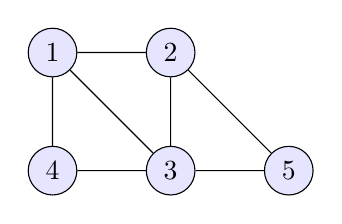
\begin{tikzpicture}[every node/.style={circle,fill=blue!10,draw,minimum size=0.5cm,node distance=1.5cm}]
        \node (1) {$1$};
        \node[right of=1] (2) {$2$};
        \node[below of=2] (3) {$3$};
        \node[left of=3] (4) {$4$};
        \path[draw] (1) -- (2) -- (3) -- (4) -- (1) -- (3);
        \node[right of=3] (5) {$5$};
        \path[draw] (2) -- (5) -- (3);
        \end{tikzpicture}
    \end{center}
    For a given $k>0$, we want to determine whether this graph has a vertex cover of size at most $k$.

    \begin{enumerate}[(a)]
        \item Choose a suitable language (a set of propositional variables) $\mathbb P$.
        \item Formalize in propositional logic the problem of whether the graph in the picture has a vertex cover of size at most $k$, for a fixed $k$. Denote the resulting theory by ${VC}_k$.
        \item Show that ${VC}_2$ has no models, i.e., the graph does not have a 2-element vertex cover.
        \item Could you use the tableau method for this? Think through the procedure.
        \item Could you use the resolution method for this? Think through the procedure.
        \item Find all 3-element vertex covers.            
    \end{enumerate}

    \begin{solution}
        A vertex cover is a set of vertices $C$ containing at least one endpoint of every edge.
        \begin{enumerate}[(a)]
            \item A natural choice is one propositional variable $p_v$ for each vertex $v\in V$, which says whether $v\in C$. Thus $\mathbb P=\{p_v\mid v\in V\}=\{p_1,p_2,p_3,p_4,p_5\}$.
            \item First, formalize that we have a vertex cover (of arbitrary size). For each edge $\{u,v\}\in E$ we express that $u$ or $v$ must be in $C$. We thus have a theory describing all vertex covers:
            $$
            VC=\{p_u\lor p_v\mid \{u,v\}\in E, u<v\}
            $$
            
            It remains to express that at most $k$ propositional variables are true, which we write as a disjunction of negations over all $(k+1)$-element subsets of vertices:
            $$
            S_{\leq k}=\{\bigvee_{v\in I} \neg p_v\mid I\subseteq V,|I|=k+1\}
            $$
            The resulting theory will therefore be $VC_k=VC\cup S_{\leq k}$.
            \item For clarity, we list all axioms of the theory $VC_2$ here (though we don’t have to):
            \begin{align*}
                VC_2=&\{p_1\lor p_2,p_1\lor p_3,p_1\lor p_4,p_2\lor p_3,p_2\lor p_5,p_3\lor p_4,p_3\lor p_5,\\
                &\neg p_1\lor\neg p_2\lor\neg p_3,\neg p_1\lor\neg p_2\lor\neg p_4,
                \neg p_1\lor\neg p_2\lor\neg p_5,\neg p_1\lor\neg p_3\lor\neg p_4,
                \neg p_1\lor\neg p_3\lor\neg p_5,\\ &\neg p_1\lor\neg p_4\lor\neg p_5,
                \neg p_2\lor\neg p_3\lor\neg p_4,\neg p_2\lor\neg p_3\lor\neg p_5,
                \neg p_2\lor\neg p_4\lor\neg p_5,\neg p_3\lor\neg p_4\lor\neg p_5\}
            \end{align*}
            Using the ‘inefficient’ approach, we can, for example, notice that:
            \begin{align*}
                \M(p_1\lor p_3,p_1\lor p_4,p_3\lor p_4,\neg p_1\lor\neg p_3\lor\neg p_4)&=\{(0,a,1,1,b),(1,a,0,1,b),(1,a,1,0,b)\mid a,b\in\{0,1\}\}\\
                \M(p_2\lor p_3,p_2\lor p_5,p_3\lor p_5,\neg p_2\lor\neg p_3\lor\neg p_5)&=\{(a,0,1,b,1),(a,1,0,b,1),(a,1,1,b,0)\mid a,b\in\{0,1\}\}\\
            \end{align*}
            These are the 2-element vertex covers of the subgraphs $\{1,3,4\}$ and $\{2,3,5\}$. Their intersection is
            $$
                \{(0,0,1,1,1),(0,1,1,1,0),(1,1,0,1,1),(1,0,1,0,1),(1,1,1,0,0)\}
            $$
            But none of these models satisfies the remaining axioms; for example, in the first one $\neg p_3\lor\neg p_4\lor\neg p_5$ does not hold.
            \item We use the tableau method to prove that $VC_2$ entails a contradiction, i.e., the formula $p_1\land \neg p_1$. We put this into the root with the marker $\mathrm{F}$ (`False’), i.e., we prove inconsistency by contradiction. We show only part of the construction (the left branch).
           
            \begin{center}
                \begin{forest}
                    [$\mathrm{F}p_1\land\neg p_1$
                        [$\mathrm{F}p_1$
                            [$\mathrm{T}p_1\lor p_2$
                                [$\mathrm{T}p_1$, tikz={\node[fit to=tree,label=below:$\otimes$] {};}]
                                [$\mathrm{T}p_2$
                                    [$\mathrm{T}p_1\lor p_3$
                                        [$\mathrm{T}p_1$, tikz={\node[fit to=tree,label=below:$\otimes$] {};}]
                                        [$\mathrm{T}p_3$
                                            [$\mathrm{T}p_1\lor p_4$
                                                [$\mathrm{T}p_1$, tikz={\node[fit to=tree,label=below:$\otimes$] {};}]
                                                [$\mathrm{T}p_4$
                                                    [$\mathrm{T}\neg p_2\lor (\neg p_3\lor \neg p_4)$
                                                        [$\mathrm{T}\neg p_2$
                                                            [$\mathrm{F}p_2$, tikz={\node[fit to=tree,label=below:$\otimes$] {};}]
                                                        ]
                                                        [$\mathrm{T}\neg p_3\lor \neg p_4$
                                                            [$\mathrm{T}\neg p_3$
                                                                [$\mathrm{F}p_3$, tikz={\node[fit to=tree,label=below:$\otimes$] {};}]
                                                            ]
                                                            [$\mathrm{T}\neg p_4$
                                                                [$\mathrm{F}p_4$, tikz={\node[fit to=tree,label=below:$\otimes$] {};}]
                                                            ]
                                                        ]
                                                    ]
                                                ]
                                            ]
                                        ]
                                    ]
                                ]
                            ]
                        ]
                        [$\mathrm{F}\neg p_1$
                            [$\mathrm{T}p_1$, tikz={\node[fit to=tree,label=below:$\vdots$] {};}
                            ]
                        ]
                    ]
                \end{forest}
            \end{center}

            (Alternatively, we could use a tableau method adapted directly to searching for models: put the validity of the first axiom at the root and expand the tableau while adding assumptions of the validity of the other axioms; every model must agree with some branch, but all of them will turn out contradictory.)
            
            \item All axioms are already in CNF. It suffices to find a resolution refutation of the theory $VC_2$ (that is, a resolution proof of the empty clause $\square$); it then follows that $VC_2$ cannot have a model. We draw only one possible resolution tree:
            
            \begin{center}
                \scalebox{0.8}{
                \begin{forest}
                    for tree={grow=north}
                    [$ \square $
                        [$ \{\neg p_1\} $
                            [{$ \{p_2\} $}
                                [{$ \{p_2,\neg p_3\} $}
                                    [{$ \{p_1,p_2\} $}]
                                    [{$ \{\neg p_1,p_2,\neg p_3\} $}
                                        [{$ \{p_2,p_5\} $}]
                                        [{$ \{\neg p_1,\neg p_3,\neg p_5\} $}]
                                    ]
                                ]
                                [{$ \{p_2,p_3\} $}]
                            ]
                            [{$ \{\neg p_1,\neg p_2\} $}
                                [{$ \{p_3\} $}
                                    [{$ \{\neg p_2, p_3\} $}
                                        [{$ \{p_1,p_3\} $}]
                                        [{$ \{\neg p_1,\neg p_2, p_3\} $}
                                            [{$ \{p_3,p_5\} $}]
                                            [{$ \{\neg p_1,\neg p_2,\neg p_5\} $}]
                                        ]
                                    ]
                                    [{$ \{p_2,p_3\} $}]
                                ]    
                                [{$ \{\neg p_1,\neg p_2,\neg p_3\} $}]
                            ]
                        ]
                        [$ \{p_1\} $
                            [{$ \{p_1,\neg p_2\} $}
                                [{$ \{p_1,p_3\} $}]
                                [{$ \{p_1,\neg p_2,\neg p_3\} $}
                                    [{$ \{p_1,p_4\} $}]
                                    [{$ \{\neg p_2,\neg p_3,\neg p_4\} $}]
                                ]
                            ]
                            [{$ \{p_1,p_2\} $}]
                        ]
                    ]
                \end{forest}
                }
            \end{center}
            

            \item Here we state just the correct answer: $\M(VC_3)=\{(0,1,1,1,0),(1,0,1,0,1),(1,1,1,0,0)\}$, which corresponds to the vertex sets $\{2,3,4\},\{1,3,5\},\{1,2,3\}$. Using the tableau method would be a bit more laborious, but you can try to prove (by the tableau method or by resolution) that vertex 3 must always be in the cover.
        \end{enumerate}
    \end{solution}

\end{problem}


\section*{Extra practice}


\begin{problem}
    
    Consider the following statements:
    \begin{enumerate}[(i)]
        \item {\it Whoever is a good runner and is in good shape will finish a marathon.}
        \item {\it Whoever is unlucky and not in good shape will not finish a marathon.}
        \item {\it Whoever finishes a marathon is a good runner.}
        \item {\it If I am lucky, I will finish a marathon.}
        \item {\it I am in good shape.}
    \end{enumerate}
    Similarly to the first example, describe the situation using propositional logic:
    \begin{enumerate}[(a)]
        \item Formalize these statements as a theory $T$ over a suitable set of propositional variables.
        \item Find all models of the theory $T$. 
        \item Try to use the \emph{tableau method} to search for models.
        \item Write several different consequences of the theory $T$.
        \item Find a CNF theory equivalent to the theory $T$.
    \end{enumerate}
    
\end{problem}


\begin{problem}

    We have three brothers; each of them either always tells the truth or always lies.
    \begin{enumerate}[(i)]
        \item The eldest says: \emph{``Both my brothers are liars.''}
        \item The middle one says: \emph{``The youngest is a liar.''}
        \item The youngest says: \emph{``The eldest is a liar.''}
    \end{enumerate}
    Using propositional logic, show that the youngest brother is truthful.
     
\end{problem}


\begin{problem}

    Consider a fixed Sudoku puzzle. Describe how to create a theory (in propositional logic) whose models correspond exactly to valid solutions.
    
\end{problem}


\begin{problem}

    Formalize the following statements in propositional logic:
    \begin{enumerate}[(a)]\it
        % \item The blueberries along the path are ripe, but rabbits in the area have not been observed.

        \item Rabbits in the area have not been observed and walking along the path is safe, but the blueberries along the path are ripe.
        
        \item If the blueberries along the path are ripe, then walking along the path is safe only if rabbits have not been observed in the area.
        
        \item It is not safe to walk along the path, but rabbits in the area have not been observed and the blueberries along the path are ripe.
        
        \item For walking along the path to be safe, it is necessary but not sufficient that the blueberries along the path are not ripe and rabbits have not been observed in the area.
        
        \item Walking along the path is not safe whenever the blueberries along the path are ripe and rabbits have been observed in the area.
    
    \end{enumerate}
    
\end{problem}


\begin{problem}

    Formalize the following properties of mathematical objects in propositional logic:
    \begin{enumerate}[(a)]
        % \item For a fixed (finite) graph $G$, that it is 3-regular.
        \item For a fixed (finite) graph $G$, that it has a perfect matching.
        \item For a fixed partially ordered set, that it is totally (linearly) ordered.
        \item For a fixed partially ordered set, that it has a least element.
    \end{enumerate}

\end{problem}


\begin{problem} 
    
    For the following formulas draw the formula tree, and find the set of models: \\(a) $(p \to q) \leftrightarrow \neg (p \wedge \neg q)$\qquad (b) $(p \leftrightarrow q) \leftrightarrow ((p \vee q) \to (p \wedge q))$

\end{problem}



\section*{For further thought}


\begin{problem}

    Recall the definition of the \emph{formula tree}.
    \begin{enumerate}[(a)]
        \item Prove in detail that every formula has a uniquely determined tree.
        \item Would this still be true if we replaced the symbols `(', `)' in the definition of a formula by the symbol `|'?
        \item What would happen if we omitted parentheses entirely?
    \end{enumerate}

\end{problem}
